\chapter{\statusgreen Common Ground Search}
\label{chap:common_ground_search}

% \todoAWinline{The point of reproducing the expt. is to determine how well their technique supports your own research aims. So this section really wants to have some quantification of the results. But also, you're interested in the qualitative question of how well you can identify those sentences which are not the basic statements of fact. So you want this chapter to lead into a discussion of how well you can identify the factual v. manipulative sentences, and the degree to which the non-factual sentences can be used to identify propaganda etc.}
% \todoHA{I agree}

% \todoHAinline{Overall, I can see a good chapter here, but need a good revision to better link the experiment with the RQs in this thesis, to detail the data used, detail the results and explain them more thoroughly, to describe the steps and rationale of the experiments more clearly (structure). And to more clearly explain the contribution beyond just replicating a previous paper.}

\section{\statusgreen Introduction}

% TODO: Research Question of this chapter
% Summary of findings / contributions
% - limitations of current methods for corroboration/omission detection
% - similarity methods ? 
% - 

% chapter motivation: multiple versions of the same story 
% This chapter contains the first set of practical experiments that we carried out.
% \todoHA{Run Grammarly on all text}
% general goal
This chapter aims to analyse how different articles present the same event from different perspectives.
For each \gls{event}, different news sources publish a big multitude of articles.
These articles can be more or less similar between them, possibly leading to a variety of linguistic forms. %\todoHA{Articles about same events does not necessarily mean you get a variety of linguistic form} 
Therefore, this is an excellent opportunity to study the relationship between the bare facts (common ground) and the additional choices that are made to try to persuade the reader of a specific opinion (as discussed in Section~\ref{ssec:lit_layers_of_info}). % (with phenomena such as framing, interpretation, manipulation, propaganda).\todoAW{How similar are these terms? Framing is much less loaded than Propaganda}\todoHA{Only mention the ones you are studying}

% fit into thesis
% But how does this fit into the overall goal of the thesis? Our overall research questions aim at studying the relationship between propaganda and political leaning (overall \acrshort{rq}1: \textbf{What is the relationship between propaganda and political leaning?}).\todoHA{Unclear how this chapter is connected to this RQ}\todomargin{general goal, and RQ1 is specific: To what extent do news articles about the same events differ?}
% But, first of all, we need to take awareness that 
% In order to study persuasion techniques as the additional layer on top of the facts (as discussed in Section~\ref{ssec:lit_layers_of_info}) we want to exploit the multitude of writings about the same topics. 
For this reason, this first experimental chapter is about parallel news reports and comparing the shared information between the articles.
% Given that the articles are a mix between raw facts and this additional layer of persuasion, %/opinion/propaganda,\todoAW{Interesting that you didn't include "framing" here...} % framing not used because it is more difficult to detect agenda setting (e.g. selecting what to include in article? But at the same time this chapter is about omission and corroboration so should be related
Considering articles coming from different news sources, that have potentially different political ideologies, we aim to extract which parts are shared and which parts are instead unique to each article.
% which part is shared and therefore is likely to be more closely related to the base layer of facts.\todoHA{?}
Relying on this analysis, we may understand the point of view of each article and how it differs from others.
%(TODO: to retake this afterwards and talk about credibility signals from bountouridis corroboration omission).
% Having this first differentiation between shared, omitted and unique, we also want to assess whether this is correlated to language that wants to persuade (propaganda). --> chapter 4 

Our experiments, therefore, are directed at automatically comparing and finding differences in similar articles, and trying to understand the reasons for articles to be different or similar.
%\todoHA{How does this fit with your RQ?}

% RQ of this chapter
For this reason, we dive into the work of spotting similarities and differences between multiple articles.
Our Research Question for this chapter is \acrshort{rq}1: \emph{To what extent do news articles about the same events differ?}
We divide it in several sub-questions: 
\begin{enumerate}[label={\textbf{RQ1.\arabic*:}},leftmargin=2cm]
    \item How are new events reported differently by multiple sources?
    \item How could we identify what is unique for each report and what is common? 
    \item To what extent can we automatically detect omission and corroboration across multiple articles?
    \item Which similarity metrics are best for detecting omission and corroboration?
    % \item What type of document/sentence encoding performs better to detect corroborations and omissions? OR What are the characteristics that allow encoding better documents and sentences?\todoAW{Is this a technical question? (ie. what's the best parser, for example?) "How can we automatically detect...?" and then expand in the main body of the text}
    % Is there a link between the parts that are different and propaganda/loaded language? --> chapter 4
\end{enumerate}



% find the shared information across several articles, and identify which parts are changed/unique. How sentences are changed between multiple articles.
% We take from the work of~\citet{bountouridis} and expand ...

% overview of subsections
In the following sections, we first give an overview of the data resources available for this task (Section~\ref{sec:cgs_data}). Next, we
analyse in Section~\ref{sec:cgs_cross_referencing} an existing approach to detect corroborations and omissions between articles. Then in Section~\ref{sec:cgs_similarity} we explore the methods to compute document similarity, and in Section~\ref{sec:cgs_clustering_and_differences} we describe our method to extract fine-grained differences at the word-level. Finally, in Section~\ref{sec:cgs_findings} we discuss our findings.

% % method
% Method: 
% hierarchical clustering of sentences, omissions/corroborations + changed parts
% Ranking of similarity by models and by me


% Findings?
% threshold of similarity challenging to find. Meaning and sentence similarity don’t always go together (all models tried)


% Limitations?



% Outline

% - cross-referencing articles (bountouridis)
% - similarity
% - sentence clustering and small differences





% \section{from upgrade report (TODO)}

% During the first year, several activities have been done.
% Some have been done as initial explorations in the field of research, understanding what other researchers have done, ``getting the hands dirty'' with data and NLP tools.
% And their function within the PhD project has been to lead to the Research Questions that we described earlier.
% Some other activities have been done to kick start the future experimentation, for example doing data collection of news articles or by beginning to implement some of the stages of the processing pipeline that will be used.
% % , with the goal to find and formulate proper Research Questions and to prepare the execution of the proposal.


\section{\statusgreen Data Resources}
\label{sec:cgs_data}
% what
% We also started collecting, early this year, several types of data that will be useful for the analysis planned.
% For this first chapter, we have been focusing on parallel news dataset. We started by using existing datasets, and then we started collecting on our own because we wanted specific features.
To analyse parallel news reports, we consider here both existing datasets, ready to be used, and also resources that we collected from scraping the public web.
% why
% The reason for this, is that 
We are interested in specific features, and existing datasets are not always having all the requirements.
First of all, a wide set of articles is needed, dense in time and from a wide variety of news outlets. We need substantial overlap between articles and the more sources we can include, the better we can observe variations of the framing phenomena.
Another very important feature is to have a good pre-clustered set of articles to help the curation of a dataset, %especially for the first Research Question, 
by knowing that the articles are well-related.
% Then, when we will have the document clustering in action, this feature is not anymore required, but still can serve as a benchmark for that stage.
If we substitute this requirement with a clustering algorithm, we need to ensure a high quality of the clusters. We decided instead to use articles that are already grouped together, to remove an additional source of issues.
A last desirable feature would be to have articles that come from sources with different opinions, such as different political ideologies. %, that would be beneficial to create examples especially for the user study, where we want to maximise the occurrence of framing techniques. 
This is because the general goal of this thesis is to study persuasion and propaganda, so if the points of view are different we can see the propaganda more easily.

% how
% - google news (more than 500k articles) daily. Some stats about the number of sources involved  TODO: how is it made? What are its properties? Why useful?
Given these requirements and after exploring different news aggregators, we found that Google Headlines Full Coverage feature\footnote{\url{https://www.blog.google/products/news/new-google-news-ai-meets-human-intelligence/}} would fit the requirements of covering a big number of news sources (the \texttt{en-GB} version contains articles from more than 10k domains) and being very dense (an average of 9k new articles each day).
The data comes divided by topics (Latest, United Kingdom, World, Business, Technology, Entertainment, Sports, Science, Health) and inside each topic, the articles are grouped into ``stories''. Each story has articles from the most relevant sources (``Top coverage'') and then also lists articles from other less important sources, for an average of 40 articles per story.
The stories are created automatically by Google News, and this makes available an enormous number of articles and sources updated continuously. %it to be always updated and be diverse in the sources included.
We captured every day, during the March–September period of 2020, the published set of stories. In this way, we managed to retrieve more than 700k articles. Not all the articles listed can be retrieved because of paywalls or other blocks by the publishers.

% - allsides: human-created with interesting framing differences
Another data source that we actively retrieve is AllSides which provides a curated set of ``headlines''\footnote{\url{https://www.allsides.com/story/admin}} where three articles with different political alignments are put together and compared in their difference.
The curators describe how the story gets framed by the considered sources, using natural language.
This description usually contains the usage of terms or themes that get mentioned.
%At the end of June, we have available 4764 headlines, with 13979 articles linked.
Differently from Google Headlines which has different versions for each country, this data is US-focused being curated in the US and therefore has a much more limited scope. Also, the discussion of bias and framing is mainly focused on political issues, while other data sources (such as Google News) are more general. %we want to focus also on other types of differences of opinion.
% role of this specific data
% This data, although the description of the differences is not directly parsable, will be used to feed the user study and understand the role of comparing different sides.

% - allnews: standard benchmark, wide adopted (find refs)

% scraping is legal for research: https://aballatore.space/2020/04/01/web-scraping-is-legal/

% % role of this
% The data collection done in these current months will continue across the PhD, and will be used in different stages of the analysis. It will serve as the seed to create the labelled dataset for the first Research Question and also provide a wide set of articles from different news sources to empower the studies of the second Research Question.
% Having articles from so many different news sources, we can on one side provide some indication of framing for news sources that are not usually targeted by manual framing studies because not enough ``important'', and on the other side be more confident to observe some phenomenon of information re-usage that is the underlying hypothesis for the last sub-question.
These two data sources are used for this and the next chapter. From Chapter~\ref{chap:political_sides} onward instead we rely mainly on an existing dataset, still coming from AllSides~\citep{baly2020we} because we want to compare our results with other works.

In this chapter, we also use \emph{All-the-news}\footnote{\url{https://www.kaggle.com/datasets/snapcrack/all-the-news}} which includes more than 140k articles published by fifteen major US outlets.
The articles are collected by using RSS feeds or collecting directly from the homepages of the news sources. The sources in question are: Atlantic, Breitbart, Business Insider, Buzzfeed News, CNN, Fox News, Guardian, National Review, New York Post, New York Times, NPR, Reuters, Talking Points Memo, Vox and Washington Post.
The articles are not balanced across news sources, as some sources were more prolific than others in the considered period.
The topics of the news are not limited to anything specific, and therefore the news articles include very different topics.


\section{\statusgreen Corroboration and Omission Extraction}
\label{sec:cgs_cross_referencing}
% Experiment 1
% what
Articles may share information, so the first step for our analysis is to identify which parts are in common and which others change.
We started by taking as reference the paper from~\citet{bountouridis2018explaining} which presents a methodology to analyse how much information overlaps between different similar documents, identifying points of information that are \gls{corroborate}[d] or \gls{omit}[ted].

The main message of the paper is that sources that \gls{corroborate} the most are also sources that get a higher ``factual reporting'' score (as measured by Media Bias/Fact Check).\footnote{\url{https://mediabiasfactcheck.com/}}
Instead, the sources that \gls{omit} the most are the ones which get a lower score.
% why
% We wanted to analyse this resource because it seems to be going in the broad direction of our project, analysing different presentations in the news of the same event.

% details about this approach, be specific that is not my work. But thesis should be standalone
The approach used by the authors is the following:
\begin{enumerate}
    \item building document-level \gls{clique}[s]: documents are encoded (using TF-IDF), the matrix of their similarity is computed, then a threshold is applied to prune the similarity relationships. Afterwards, a graph is produced where the nodes are documents and the edges are the similarity relationships that satisfy the minimum threshold. This graph is then processed to identify the cliques and the outputs are then filtered to enforce that every document only belongs to one clique. Each clique represents a story that was covered by multiple documents (because they are similar between them). Not all the documents belong to a clique, they can be left out;
    \item building sentence-level \gls{clique}[s]: starting from the document-level cliques of the previous step (same story), each one of them is considered on its own, and the articles are split into sentences. Then, all the sentences are processed as in the previous step (encoding representation, similarity computation, similarity threshold, cliquing algorithm, clique post-processing). The outputs are sentence-level cliques that represent a piece of specific information that appears in multiple documents; 
    \item computing outlet-related corroboration and omission: sentence-level cliques are grouped by publishing outlet; then omitted cliques (appearing in other outlets but not in the considered one) and corroborated cliques (also appearing in other outlets) are counted;
    \item analysing correlation with factuality scores: the ratios of omitted cliques and corroborated cliques are compared with the scores coming from Media Bias/Fact Check for each outlet, and the hypothesis of correlation is verified: corroboration appears more in factual sources, while omission appears more in non-credible sources.
\end{enumerate}

% dataset
The dataset used is the \emph{All-the-news}\footnote{\url{https://www.kaggle.com/datasets/snapcrack/all-the-news}} which includes more than 140k articles published by fifteen major US outlets. To have the same results as the reference paper~\citep{bountouridis2018explaining}, we reproduce the paper by using only articles from 2016. This brings the analysis to work with 203 document-level cliques. 

% how
We analysed and reproduced this paper to get a deep understanding of how it works, and to extend its methodology to analyse the word-level differences. %\todoHA{Expand: anything else to be discovered?} 
The implementation started with the code and data %\todoAW{What are the properties of the dataset?} 
publicly provided by the authors,\footnote{\url{https://github.com/dbountouridis/InCredible}} but its incompleteness in some stages of the processing (e.g., the creation of the document-level cliques, and all the specific hyperparameters of the algorithms used) required integrating the codebase.\footnote{\url{https://github.com/MartinoMensio/InCredible}}

\begin{figure}[!htbp]
    \centering
    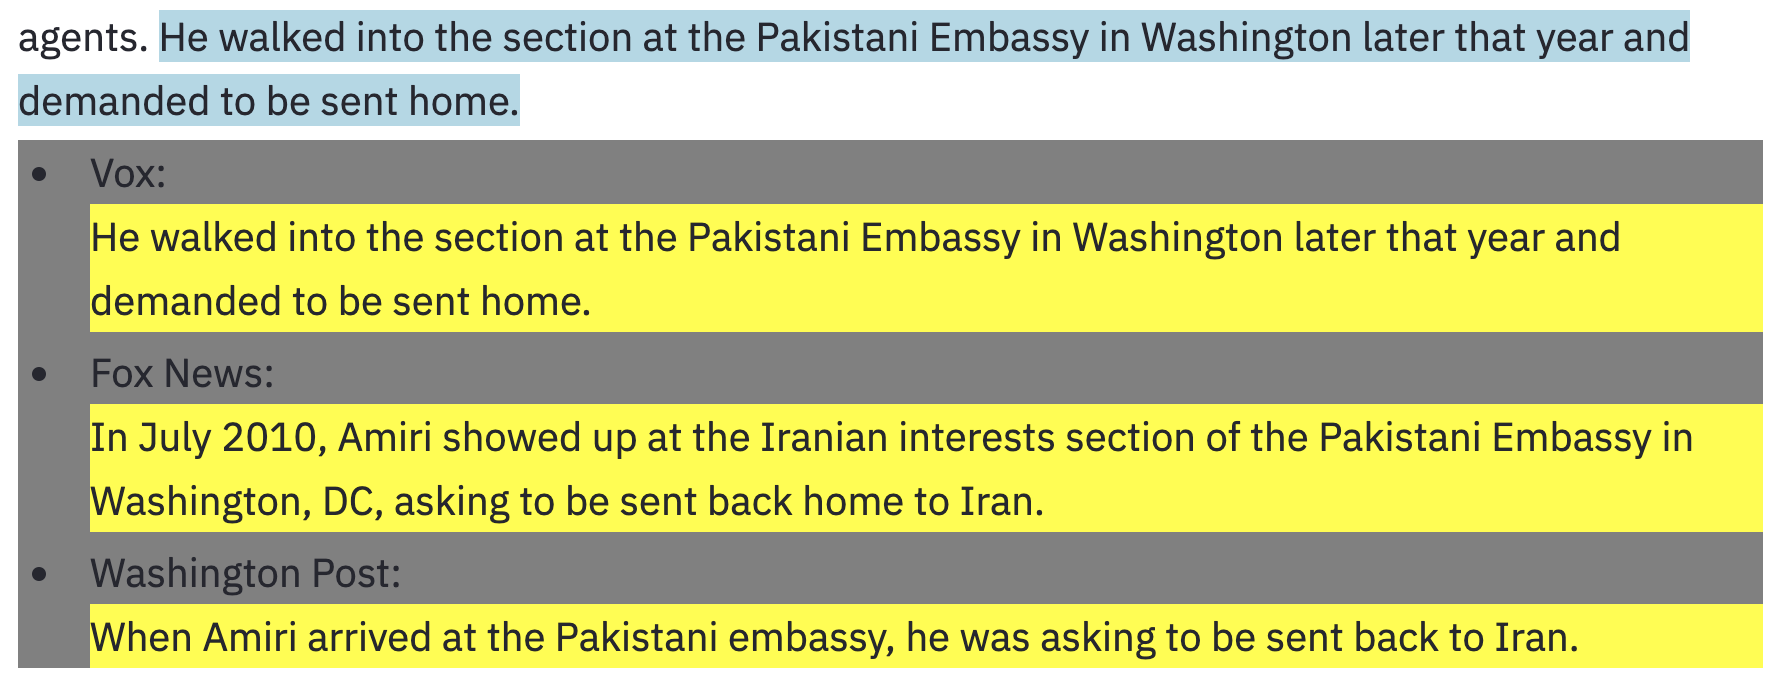
\includegraphics[width=\linewidth]{figures/cluster_similar_sentences_amiri.png}
    \caption{Corroboration example between Vox, Fox News and Washington Post.}
    \label{fig:cluster_similar_sentences_amiri}
\end{figure}%\todoHA{Good to have an example. But unclear what is the output, what did you get when processed these examples?}

An example of the reproduced analysis can be seen in Figure~\ref{fig:cluster_similar_sentences_amiri}.
In this example, the step 1 identified an article-level clique of 3 articles (Vox, Fox News, Washington Post) that cover the connection between Hillary Clinton's email and Amiri Shahram being executed.\footnote{\url{https://www.vox.com/2016/8/9/12410882/clinton-emails-trump-iranian-scientist-executed-amiri}}
The step 2 instead, identifies the three specific sentences that cover the detail of Amiri at the Pakistani Embassy in Washington.
Step 3 counts these sentences as corroboration between Vox, Fox News and Washington Post. 

\begin{figure}[!htbp]
    \centering
    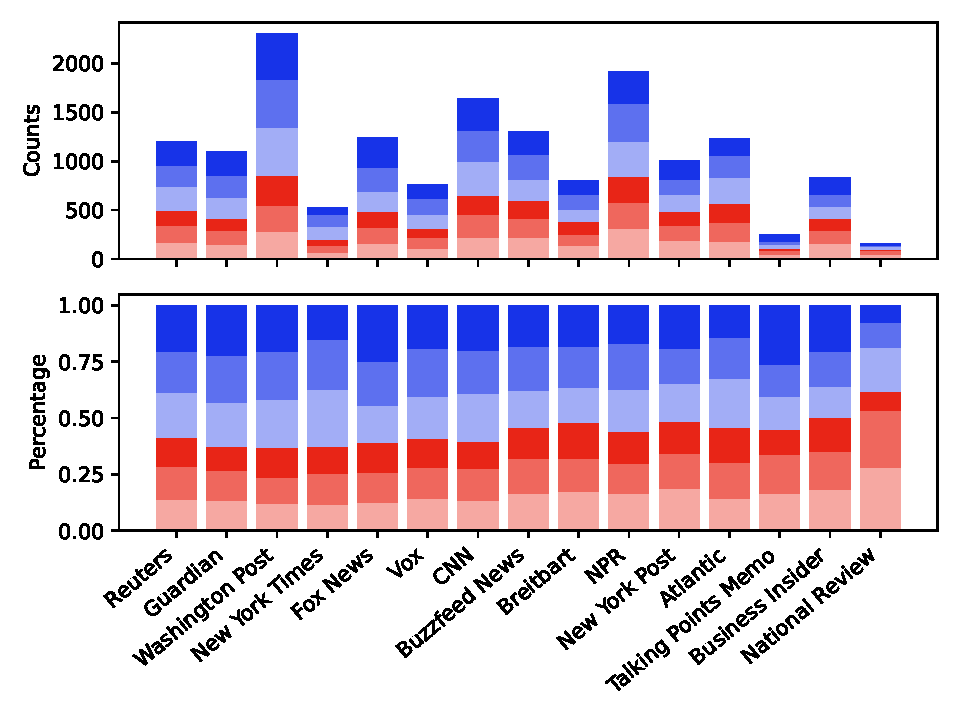
\includegraphics[width=\linewidth]{figures/bountouridis_fig_3_noGA.pdf}
    \caption{Corroborated (blue) and omitted (red) sentences per news outlet.}
    \label{fig:figure_3_bountouridis_reproduced}
\end{figure}%\todoHA{Do you point to this from anywhere?}

Figure~\ref{fig:figure_3_bountouridis_reproduced} shows our reproduction of the source-level corroboration and omission counts (top) and percentages (bottom).
Colour shading (quantised to three bins) indicates the average TF-IDF similarity among the sentences in cliques, i.e. the lighter the shade, the more dissimilar. This plot is almost identical to the one originally contained in~\citet{bountouridis2018explaining}, meaning that we reproduced correctly the complete approach.



% limitations
With the experiments and the interactive visualisation reproduced, we have been able to manually inspect the cliques of documents. For each of the 203 cliques of documents, we manually checked whether all the articles were topically related, and we observed that in 20\% of the cases, the document-level cliques were too wide (including articles from another main event) or too narrow (multiple cliques should have been merged together.
For a small portion (20 cliques), we inspected the sentence-level cliques to understand how similar the sentences were, and what types of differences they contained.
We identified the following limitations:
% and sentences identified by the model, seeing the following limitations:\todoHA{How? Method? How many? Give proper numbers}

\begin{itemize}
    % \item Their demo\footnote{\url{http://fairnews.ewi.tudelft.nl/InCredible/}} just shows one specific article as main and one specific clique (not very interesting)
    \item The \emph{document cliquing}
    %\todoAW{You've jumped very suddenly into the use of particular algorithms. What are these algorithms doing? How do you interpret their output? Are they your implementation or Bountouridis et al's? etc} 
    sometimes splits similar articles over different groups, or in some cases has different stories that talk about a different detail within the same clique (e.g., when a news story re-emerges because further details are discovered).
    This can be a consequence of having TF-IDF as the underlying method to represent the documents.
    This method is fast and efficient for coarse topic detection because, being based on bag-of-words, works well with specific terms that distinguish the topics.
    But when we need to have a finer-grained clustering such as in this case, the limitation of this method may surface: the terms of two political events with the same entities mentioned result in having similar feature vectors.
    It is not enough to change the thresholds to obtain better document cliques.
    \item The \emph{sentence cliquing} method provided just uses the degree of similarity between two sentences but does not point to which specific words are responsible for the similarities and differences. This would require a fine-grained analysis that in this paper is not included. Furthermore, sentences in a clique are very similar, and no significant differences have been observed because the similarity metrics are based again on TF-IDF. This method is not robust enough to the usage of synonyms and other variations on the linguistic surface, while at the same time is unable to distinguish two sentences that use the same words but have different meanings. These different meanings may be caused by the sentence structure or the role of the words. Therefore, selecting a threshold value becomes very difficult.
    \item The \emph{clique algorithms} are not the best choice for grouping when we have the information of how much similar two items are (a real-value instead of a binary-value is available from the similarity metric). The approach considers an unweighted version of the similarity graph by using a threshold (weights are just used to select the most appropriate clique during their creation). Instead, if we use the original weighted graph, we can use better and more flexible clustering techniques (e.g., agglomerative clustering). %, like agglomerative clustering
\end{itemize}
% \todoHA{All this is interesting but not very clear how you reached these conclusions and what they signify}





% In addition to these problems, the model described is based on TF-IDF which is not as robust with changes on the linguistic surface (as we saw in the next experiment).
% Models flourished
% This is the motivation for 5.1.2

% And also, it uses the similarity between TF-IDF just with a threshold, modelling the graph and cliques as unweighted (the weights are just used to select the most appropriate clique during their creation).

% role of this experiment
Reproducing this experiment helped us to see the limitations of this work. %, which belongs to the \emph{similarity} area of research (Section~\ref{sec:lit_relationships}).
This paper provides a great way to analyse the overlap between articles and extracts pieces that have been omitted or that are corroborated, but does not investigate further the reason behind the selection of what is included or not.
This opens up for further work:
\begin{enumerate}
    \item investigate how to represent the documents better to provide meaningful similarity metrics at the document and sentence level (Section~\ref{sec:cgs_similarity}); %\todoHA{Similarity of what? Why need it?}
    \item experiment with document and sentence clustering to bring up fine-grained differences. To understand the choice of terms, we first need to be able to identify how uniquely or commonly the terms are used across news articles that cover the same story(Section~\ref{sec:cgs_clustering_and_differences}); %e.g. how specific terms are chosen\todoHA{Where? Why?} (Section~\ref{sec:cgs_clustering_and_differences});
    % \item investigate the works that analyse framing theories and detection;
    \item investigate the reason for such differences to exist. This will be done in the next Chapter~\ref{chap:linguistic_persuasion} about detecting linguistic means of persuasion.
    % \item collect data from more recent articles that would be more relevant and interesting.
\end{enumerate}
% \emph{i)} , \emph{ii)} , \emph{iii)} , and \emph{iv)} g.

% Apart from these limitations, we are building our processing pipeline on top of this type of analysis, that links together news articles at different granularity levels (documents, sentences, words).
% This gives us the opportunity to use features from multiple articles for the next stage of automated detection of framing techniques.
This method of comparison has its main limitations in the similarity metric chosen. So we opted for doing some further research on the similarity metrics, in a way that accounts more for semantic similarity instead of just being term-based.


\section{\statusgreen Models for Similarity Analysis}
\label{sec:cgs_similarity}
% Experiment 2
% what
Since our biggest problem is representing documents and sentences in a way that captures more semantic similarity, we decided to analyse the existing works, including word embeddings and language models.
We wanted to see in practice how the usage of different representation models would affect the measurements of similarity, experimenting with a small set of articles. 
% finding and exploring more advanced methods to find the similarity between texts by using language models, we experimented on how to use these methods.

% why?
% is a pillar\todoHA{Too strong} for 
To compare different articles, we need to have a
solid base for computing the distances between them as a whole or more detailed to the sentence level.
The applications of similarity range from document clustering to the identification of omitted pieces of information in a cluster, therefore it is very important to use a method that is properly not deceived by the usage of synonyms and other linguistic variations in communicating the same information. To study the differences, we first need to be able to tell whether two pieces of text are discussing the same information, and distinguish degrees of similarity properly.

To study the similarity metrics, we perform an experiment in Subsection~\ref{ssec:cgs_similarity_qualitative}, where we observe qualitatively the effects of using one similarity metric or others when comparing sentences. 
% To study the similarity metrics, we use two different experiments. The first is detailed in Subsection~\ref{ssec:cgs_similarity_qualitative}, where we observe qualitatively the effects of using one similarity metric or others when comparing sentences. 
%The second instead, in Subsection~\ref{ssec:cgs_similarity_cliques}, observes the effect of such choice on the downstream task of corroboration and omission extraction.
We conclude with some observations in Subsection~\ref{ssec:cgs_similarity_conclusion}.


\subsection{\statusgreen Qualitative Differences Benchmark}
\label{ssec:cgs_similarity_qualitative}
% how?
% Specifically on the sentence level, we experimented to see how different models were able to pick similar sentences, by setting up a small benchmark.
We set up a small benchmark where the goal is to find the most similar pairs of sentences coming from selected pairs of news articles which cover the same event. Each model candidate has to tell which ten most similar pairs of sentences it has found, one from one article and one from the other.
We choose pairs of articles manually, %\todoHA{By whom?}
by considering three constraints: \textit{i)} description of the same event, \textit{ii)} from different news outlets, \textit{iii)} published near in time, with a maximum time distance of one day.
Each model extracts the most similar pairs, and we then compare the pairs provided and their relative order in the rankings.

The selected models used in the benchmark are the following:
\begin{itemize}
    \item \textbf{TF-IDF}: with a feature size of 2000, with a preprocessing made of lowercasing and tokenizing, without lemmatising;
    \item \textbf{GloVe-average}: considering GloVe word embeddings~\citep{pennington2014glove} trained on the CommonCrawl dataset, and doing an average of the vectors over the sentence;\footnote{\url{https://spacy.io/models/en\#en_core_web_lg}}
    \item \textbf{\acrshort{bert}}: using the most popular embeddings provided by Google Research~\citep{devlin2018bert} with the base uncased pre-trained weights;\footnote{\url{https://spacy.io/models/en-starters\#en_trf_bertbaseuncased_lg}}
    \item \textbf{\acrshort{use}}: using sentence embeddings coming from \acrfull{use}~\citep{cer2018universal} which has been specifically trained for sentence similarity.\footnote{\url{https://tfhub.dev/google/universal-sentence-encoder/}}
\end{itemize}

In all the cases, the representations from these models are compared with the cosine similarity.

The data follows this processing:

\begin{enumerate}
    \item articles are collected from our Google News processing described in Section~\ref{sec:cgs_data};
    \item pairs of articles are manually selected according to the three constraints listed above (1: checking that they cover the same event, 2: from different news outlets, 3: published near in time) to build a small dataset made of 20 article pairs;
    \item each article is split into sentences;
    \item each sentence is encoded with each of the models listed above;
    \item for each model and each article pair, we build a ranking of pairwise sentence-similarity (one sentence from one article and the other sentence from the other article);
    \item for each sentence-pair that appears at least in the top-10 of two rankings, we manually inspect the differences and we qualitatively describe what changes between the sentences;
    \item we compare the rankings given by the different models together with our qualitative descriptions.
\end{enumerate}


% For each pair of sentences that was provided by any of the models, we listed by manual analysis which differences were contained, in terms of details that changed, or different words used.\todoHA{The dataset used is not clearly described}

\begin{table}[!htbp]
    % \begin{subtable}[h]{\textwidth}
        \centering
        \begin{tabular}{r | p{0.4\linewidth} | p{0.4\linewidth} }
        Index & Article 1 (BBC) & article 2 (Sky News) \\
        \hline
        0\vspace{-2px} & \tiny{A 52-year-old man has been charged with the murder of journalist Lyra McKee in Londonderry.}\vspace{-2px} & \tiny{A man has been charged with the murder of journalist Lyra McKee in Northern Ireland.}\vspace{-2px}\\
        1\vspace{-2px} & \tiny{He is also charged with possession of a firearm with intent to endanger life and professing to be a member of a proscribed organisation.}\vspace{-2px} & \tiny{Ms McKee, 29, was shot dead by dissident republicans as she observed rioting in Derry/Londonderry last year.}\vspace{-2px}\\
        2\vspace{-2px} & \tiny{Ms McKee, who was 29, was observing rioting in Derry's Creggan estate when she was shot on 18 April 2019. }\vspace{-2px}& \tiny{She was standing near a police vehicle when she was hit by a bullet fired by a masked gunman towards officers.}\vspace{-2px}\\
        3\vspace{-2px} & \tiny{The 52-year-old, who is from Derry, is due to appear at Londonderry Magistrates' Court on Thursday.}\vspace{-2px} & \tiny{The so-called New IRA said it carried out the killing, which took place on the Creggan estate on 18 April.}\vspace{-2px}\\
        4\vspace{-2px} & \tiny{Det Supt Jason Murphy said a number of individuals were involved with the gunman on the night Ms McKee was killed.}\vspace{-2px} & \tiny{It said Ms McKee was caught in the line of fire while standing with what the organisation called "the enemy".}\vspace{-2px}\\
        5\vspace{-2px} & \tiny{"And while today is significant for the investigation the quest for the evidence to bring the gunman to justice remains active and ongoing," he added.}\vspace{-2px} & \tiny{The 52-year-old suspect was arrested on Tuesday and taken to Musgrave Serious Crime Suite in Belfast.}\vspace{-2px}\\
        6\vspace{-2px} & \tiny{Ms McKee was a writer and campaigner from Belfast who had only recently moved to Derry when she was killed.}\vspace{-2px}& \tiny{He has also been charged with possession of a firearm with intent to endanger life and professing to be a member of a proscribed organisation.}\vspace{-2px}\\
        7\vspace{-2px} & \tiny{She was standing near a police 4x4 vehicle on the night of 18 April 2019 when a masked gunman fired towards officers and onlookers.}\vspace{-2px} & \tiny{The Police Service of Northern Ireland said the man, who comes from the city, is due to appear at Londonderry Magistrates' Court on Thursday.}\vspace{-2px} \\
        8\vspace{-2px} & \tiny{Regarded by many as a rising star in Northern Ireland media circles, she had written for many publications, including Buzzfeed, Private Eye, the Atlantic and Mosaic Science.}\vspace{-2px} & \tiny{Detective Superintendent Jason Murphy said: "I have always said a number of individuals were involved with the gunman on the night Lyra was killed.}\vspace{-2px} \\
        9\vspace{-2px} & \tiny{She was named Sky News young journalist of the year in 2006 and Forbes Magazine named her as one of their 30 under 30 in media in Europe in 2016.}\vspace{-2px} & \tiny{"And while today is significant for the investigation the quest for the evidence to bring the gunman to justice remains active and ongoing."}\vspace{-2px} \\
        10\vspace{-2px} & \tiny{The Belfast woman had signed a two-book deal with the publisher Faber and Faber, with her forthcoming book The Lost Boys due out this year.}\vspace{-2px} & \tiny{The gay rights activist, who lived with her partner Sara Canning, was an advocate of a new and more tolerant Northern Ireland.}\vspace{-2px} \\
        11\vspace{-2px} & \tiny{According to those who knew her best, the gay rights advocate was someone who "believed passionately in social and religious tolerance".}\vspace{-2px} & \tiny{Ms McKee's death sparked widespread revulsion and a renewed effort to restore a power-sharing agreement in Stormont following years of political instability in the country.}\vspace{-2px} \\
        12\vspace{-2px} & \tiny{Her death caused widespread revulsion in Northern Ireland and further afield.}\vspace{-2px} & \tiny{Her funeral was attended by then prime minister Theresa May, Irish PM Leo Varadkar and Irish President Michael D Higgins at St Anne's Cathedral in Belfast.}\vspace{-2px} \\
        13\vspace{-2px} &  & \tiny{At her service in April last year, the priest confronted politicians, saying: "Today we grieve but tomorrow let us fill that hole by adopting Lyra's spirit, example and vision.}\vspace{-2px} \\
        14\vspace{-2px} &  & \tiny{"Let us put false starts behind us and once and for all build an alternative Ulster that we, and especially our children, can be proud of.}\vspace{-2px} \\
        15\vspace{-2px} &  & \tiny{"Let us make the lasting legacy of Lyra McKee that peace."}\vspace{-2px} \\
        16\vspace{-2px} &  & \tiny{Days later, the British and Irish governments announced a new talks process aimed at restoring devolution.}\vspace{-2px} \\
        17\vspace{-2px} &  & \tiny{Power-sharing was restored at Stormont last month and the first same-sex marriage in Northern Ireland took place this week.} \vspace{-2px}
       \end{tabular}
       \caption{Sentences from two reference articles.}
       \label{tab:sentences}
    % \end{subtable}
\end{table}
% \todoHA{How found?}



\begin{table}[!htbp]
    % \hfill
    % \pagebreak
    % \begin{subtable}[h]{\textwidth}
        \centering
        \begin{tabular}{@{\hspace{-2cm}}r | r | p{0.55\linewidth} |p{0.1\linewidth}|p{0.1\linewidth}|p{0.1\linewidth}|p{0.1\linewidth}}
        id\_1 & id\_2 & Qualitative description of differences & TF-IDF & GloVe & BERT & USE \\
        \hline
        1 & 6 & \tiny{Verb tense} & 1st 0.9707 & 1st 0.9973 & 1st 0.9835 & 1st 0.9668 \\
        5 & 9 & \tiny{“He added” at the end} & 2nd 0.9638 & 2nd 0.9954 & 2nd 0.9563 & 2nd 0.9581\\
        0 & 0 & \tiny{Details just on one article (52-year-old). Different level of detail (Londonderry vs Northern Ireland)} & 3rd 0.6858 & 4th 0.9535 & 4th 0.8972 & 3rd 0.9141\\
        4 & 8 & \tiny{Abbreviations (Dept Supt vs Detective Superintendent). Direct reporting vs paraphrasing: quotation marks and colon. “I have always said” just on one article. “Ms McKee” vs “Lyra”} & & 6th 0.9463 & 3rd 0.9244 & 4th 0.8279\\
        3 & 7 & \tiny{Subject of reporting just on sent\_2 “The Police Service of Northern Ireland said”. Detail on the man “the 52-year-old” vs “the man”. “Is” vs “comes” from. “Derry” vs “the city”} & & 5th 0.9509 & 7th 0.8533 & 5th 0.7490\\
        7 & 2 & \tiny{Detail “4x4” just on first one. Detail “on the night of 18 April 2019”. Active vs passive sentence “a masked gunman fired towards” vs “she was hit by a bullet fired by a masked gunman towards”. Detail “a bullet” vs just the “fired” verb. “Towards officers and onlookers” vs “towards officers”: in the second, the target of the gunman are just officers.} & 6th 0.6557 & 3rd 0.9550 & 12th 0.8313 & 6th 0.7254\\
        2 & 1 & \tiny{Age reporting a bit different “who was 29” vs “29”: the first has emphasis on the past tense (underlines she is dead now). Inversion of parts of the sentence: “was observing rioting when she was shot” vs “was shot as she observed rioting”. Verb tense “was observing rioting” vs “she observed rioting”. Place details “Derry’s Creggan estate” vs “Derry/Londonderry”. Shooter declared in the second one “dissident republicans”. Date details “18 April 2019” vs “last year”} & 4th 0.6782 & 9th 0.9180 & 9th 0.8487 & 7th 0.6009 \\
        12 & 10 & \tiny{Delegation of who said it: “according to those who one her best” in the first sentence and then the quotation marks. “Advocate” vs “activist”+”advocate”: the first one does not say “activist”. Sentence 2 adds the incise “who lived with her partner Sara Canning”. Quoted part “believed passionately in social and religious tolerance” vs “advocate of a new and more tolerant Northern Ireland”: (First is stronger “believed passionately”, Second is narrower “Northern Ireland”, “Social and religious tolerance” vs “more tolerant”)} & & 7th 0.9282 & 6th 0.8538 & 8th 0.5863

        \end{tabular}
        \caption{Differences and relative rankings from models.}
        \label{tab:relative_ordering}
     % \end{subtable}
     % \caption{Example of quantification of qualitative analysis
     % table with example sentences and ranking showing USE is better
     % }
     % \label{tab:temps}
\end{table}

Table~\ref{tab:sentences} shows an example of article-pair where each article has been split into sentences.
The first article is from BBC\footnote{\url{https://www.bbc.co.uk/news/uk-england-hereford-worcester-51791346}} and the second one from Sky News,\footnote{\url{https://www.dailymail.co.uk/news/article-8088805/Britons-facing-heavy-downpours-four-inches-rain-50mph-winds-set-batter-UK.html}}.
We assign an increasing index to the sentences, and we use this to identify the sentences in the next Table~\ref{tab:relative_ordering}. In this second table, we show, next to the indexes of the considered pair of sentences, the qualitative description that we manually annotated, and the rankings from the four models considered.


We created a visualisation to help compare the word-level similarity and alignment between two sentences. Figure~\ref{fig:lyra} shows this tool applied on sentence 7 from BBC and sentence 2 from Sky News (sentence indexes from Table~\ref{tab:sentences}).
% The differences are the following:

% \begin{itemize}
%     \item the detail ``4x4'' just appears on the BBC article;
%     \item the detail ``on the night of 18 April 2019'' just appears on the BBC article;
%     \item Active vs passive sentence ``a masked gunman fired'' vs ``she was hit by a bullet fired by a masked gunman'';
%     \item the detail ``a bullet'' just appears in the Sky article;
%     \item ``Towards officers and onlookers'' vs ``towards officers'': in the second, the targets of the gunman are just the officers.
% \end{itemize}

\begin{figure}[!htbp]
    \centering
    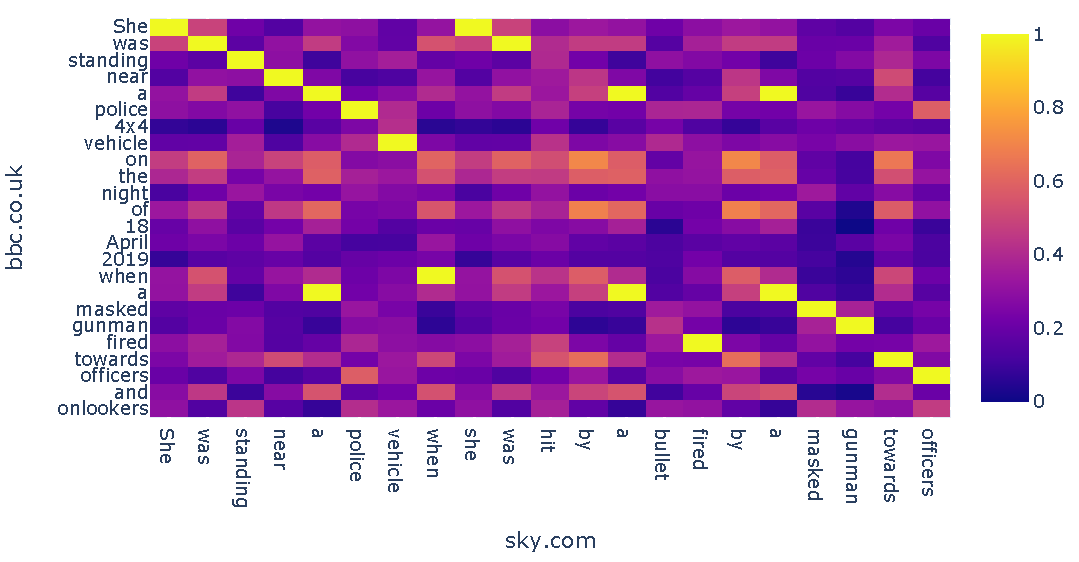
\includegraphics[width=0.9\linewidth]{figures/lyra.pdf}
    \caption{Difference analysis across similar sentences from BBC and Sky News.}
    \label{fig:lyra}
\end{figure}
% \todoHA{Table 3.2 and 3.3 refer to from text and explain}


With this kind of information on the number, type and magnitude of changes contained in different pairs of sentences, we can get a qualitative idea of how the measures of similarity coming from the different models are representative of the effective differences.
If we have two pairs of sentences, and the first pair contains bigger differences (count, magnitude) than the second one, we want the second pair to be ranked as more similar than the first one.
Therefore, if the model ranks the first pair of sentences as more similar than the second pair, that is a negative sign for that model. %\todoHA{And then what?}
% If a model scores more similar a pair of sentences that appear to us to be less related than another pair,\todoAW{Disturbingly vague!!} that is a negative sign for that model.
We can therefore understand how good the models are to rank the similarity of sentences, and make an informed decision about which model to consider for our work.


% Observations
% \todo{rewrite better the observations}
The main problem observed for the TF-IDF model is that it relies just on the terms. If two terms are interchangeable/synonyms, they are still considered as two distinct features. This is a big limitation considering that we are dealing with a wide multitude of documents,  %that deal with the same underlying events,
therefore we expect a big variance on the linguistical surface.
Then we have other technical observations for the TF-IDF model, for example, that the results change a lot depending on the feature size.
Furthermore, it requires to be computed on a set of documents all together (which also changes which features are selected), and it is not possible to encode an additional document without changing the representation of the already encoded documents because the term overall frequencies change.
We also see that the type of pre-processing affects the results: without a lemmatization step to the pipeline, it is sufficient to change the verb tense to have a different term.
Given these limitations, we find that sentences that are very similar in meaning but have some differences in the linguistic surface see a drop in their similarity with this model.

Instead, considering GloVe-average, we observe in some cases that the measure of similarity provided does not capture substantial changes in the meaning. The problem is that, while it can use wordwise similarity quite well, the sentence structure is not accounted for its representation. The representation is a simple average of the word vectors (e.g. ``Luke insulted John'' results in being equal to ``John insulted Luke''). %\todoAW{So this is a well known issue with VSM in general. How significant is it for the specific case you're looking at here?}
In our case, we need to be sensible to changes in the meaning even when the same words are used. The order of words may convey a different meaning and we want the similarity metric to capture this information.

For the language models (\acrshort{bert} and \acrshort{use} models), we see that the order given by the models is more aligned with what we consider to be the differences to be (second column of Table~\ref{tab:relative_ordering}).
What we do with this experiment is to try to make measurable something that is very qualitative (the similarity between sentences).
There exist already different benchmarks that are performed on the semantic similarity task~\citep{conneau-kiela-2018-senteval,chandrasekaran2021evolution}, and this experimentation is not trying to replicate them. Here we simply want to see how the different families of models compare on our task, where we need to understand the degree of similarity between related sentences and documents.

% a big improvement\todoAW{I'm not entirely sure at this point how you're evaluating the various methods} in the pairs of sentences that come as more similar.
% The values provided are very similar. This per-se is not a problem if some geometric properties are valid (ordering, proportions)
% We observe\todoHA{Many "observations" made here, but unclear how. Add some details if you can} that \acrshort{use} provides values less skewed to the higher end, distributing the similarity values more evenly.
Between USE and BERT, Table~\ref{tab:relative_ordering} shows that USE provides values less skewed to the higher end, distributing the similarity values more evenly. 
This is something very positive, because we want a metric that is able to tell degrees of similarity with a good granularity in all of the range.
% The numbers make more sense without any re-scaling technique, and therefore the heatmaps shown in this document\todoHA{?} come from this model.
We can directly use the values to produce heatmaps, without the need to re-scale the values. With BERT, it would be necessary as the values are all compressed in the higher end (near 100\% similarity).
Furthermore, USE is also the only model, among the four considered here, that is purposely trained on a semantic similarity task, while the other models can provide similarity measures just because of how they represent language.


% \todo{an example of two pairs where we can see some of the limitations?}

\begin{comment}
\subsection{\statusred Application to corroboration and omission extraction}
\label{ssec:cgs_similarity_cliques}
% Cliques with USE

\todo{This section needs some work still. Or otherwise remove it. Is it crucial to have this experiment?}
\todoHA{Can't tell yet. THe workflow of your thoughts and experiments need more clarification upfront in this chapter}

In this section, we take the experiment from Section~\ref{sec:cgs_cross_referencing} and substitute the TF-IDF encoding method with a semantic similarity model (\acrshort{use}).

While in the previous Subsection~\ref{ssec:cgs_similarity_qualitative} we were assessing the quality of USE vs TF-IDF on their own, here we see the difference when applying them to downstream tasks.


\todo{Show figure with USE, that results are better correlated?}

In figure\ref{fig:usebetter}, we can see that when we compare the base model TF-IDF with USE, we get a better correlation between corroboration and credibility.
% OR: we get unclear results.
% However, 
Show cliques inspection quality
when inspecting the cliques, we see that 

\todo{need an example}
\end{comment}

\subsection{\statusgreen Similarity Analysis Findings}
\label{ssec:cgs_similarity_conclusion}
% \todo{rename subsection or remove?}

% role of this experiment
This experiment shows the need for a similarity model that accounts for the semantics more than the linguistic surface. Given the continuous progress of language models, we need to be able to switch our choices relatively easily.
For example, by looking at the Semantic Textual Similarity benchmark,\footnote{\url{http://nlpprogress.com/english/semantic_textual_similarity.html}} at the moment the best model available is XLNet~\citep{yang2019xlnet} but this could change at any time.

For this reason, our following experiments use the USE model instead of the latest available models. The difference is not very big and we have the advantage of being able to compare our experiments without re-running all of them when a new model is released.

\acrshort{use} and XLNet both belong to the same family of models, so the differences between them should not be a big limitation of this work.

%so we will use it for our future experiments.
% this means for us:
% - we need to use a similarity resistant to changes in the linguistic surface
% - we need a measure that is able to represent well the different levels of similarity
% - we must be able to switch the model used easily, in case new public benchmarks for STS show a different winner (example XLNet~\citep{yang2019xlnet}).

%The purpose of this experiment is to have a good observation of how different types of models can be effective or not, and to experiment with them to drive the implementation of the processing pipeline.
% Benchmark, availability of code and maybe further measures on our system will decide the final ``winner''.
% Purpose: implementation and building of the pipeline.


\section{\statusgreen Fine-grained Differences Extraction}
\label{sec:cgs_clustering_and_differences}

% Experiment 3
% what
This section has two goals: 1) to improve the cliquing approach used in Section~\ref{sec:cgs_cross_referencing} and 2) to take a closer look at the fine-grained differences between highly-similar sentences and study the uniqueness of the words used.

% The next experimentation that we have done regards the usage of the similarity values to group together sentences describing the same details and at the same time study the uniqueness of the words used.

\subsection{\statusgreen Hierarchical Sentence Clustering}
\label{sec:cgs_clustering_and_differences_hierarchical}


% why
We have seen with the reproduction of the model from \citet{bountouridis2018explaining} that one big limitation of using cliquing techniques over unweighted graphs is that they do not exploit the full power of the distances available. This resulted in having fragmented clusters because the choice of the threshold is very sensible.
% We have also experimented with different embedding models and we want to use them
% \todo{from here on}
% This comes from the limitation of the first experiment of reproduction of the paper. (from experiment 1)
% (from experiment on similarity)

% how
With the idea to use clustering algorithms instead, we retrieved some groups of articles that relate to the same event from Google Headlines, which aggregates and clusters together news articles from multiple sources.\footnote{\url{https://www.blog.google/products/news/new-google-news-ai-meets-human-intelligence/}}
These documents are processed with the SpaCy NLP Python library\footnote{\url{https://spacy.io/}} to split the documents into sentences and have available different NLP functions (e.g., tokenisation, POS tagging).

% 1. distance computation
Each of the sentences is then passed through a language model which creates a sentence embedding, in this case using \acrshort{use} because it showed to distribute the similarity values more evenly and is specifically trained for sentence similarity.

% 2. hierarchical clustering (example with diagram)
We then use \acrfull{hac} for different reasons:
\begin{itemize}
    \item it does not require the specification of the number of clusters wanted, we want to be flexible;
    \item we can truncate the clustering when we reach a certain level of distance between the clusters, or a certain number of clusters;
    \item We can see the evolution of many different features (e.g., number of clusters, size, internal cohesion) while performing the clustering step by step;
    \item we have a graphical representation (dendrogram) which helps to inspect and understand what is happening;
    \item it has widely been used for similar tasks, e.g., finding related claims~\citep{almeida2020text}
\end{itemize}

% This clustering algorithm has the following parameters:
% \begin{itemize}
%     \item linkage method: how to choose which clusters to merge. Different strategies exist: Ward: minimise the total within-cluster variance (weighted squared distance between cluster centres). Single: Nearest Point Algorithm. Complete: Farthest Point Algorithm
%     \item distance function: cosine, euclidean, ...
% \end{itemize}
% \todo{describe why ward and cosine look better}

For this experiment, we consider a total of 20 different headlines, with an average size of 70 articles each.
After splitting the sentences, we have an average of 33 sentences for each article (total of 46373 sentences).
The \acrshort{hac} is done for each headline separately.

In Figure~\ref{fig:dendrogram}, we can see how different thresholds for sentence similarity would affect the generated clusters. The dendrogram on the right shows which sentences get in the same cluster at increasing distance values. Identical sentences are merged at the left of the dendrogram, with similarity close to $0$, while totally different groups of sentences get merged with higher values (near $1$ considering cosine distance).
% what is the distance required to have different sentences inside the same cluster,
%\todoHA{How these links were detected? How many sentences processed? Links context? Etc.} and select a certain threshold more consistently.
\begin{figure}[!htb]
    \centering
    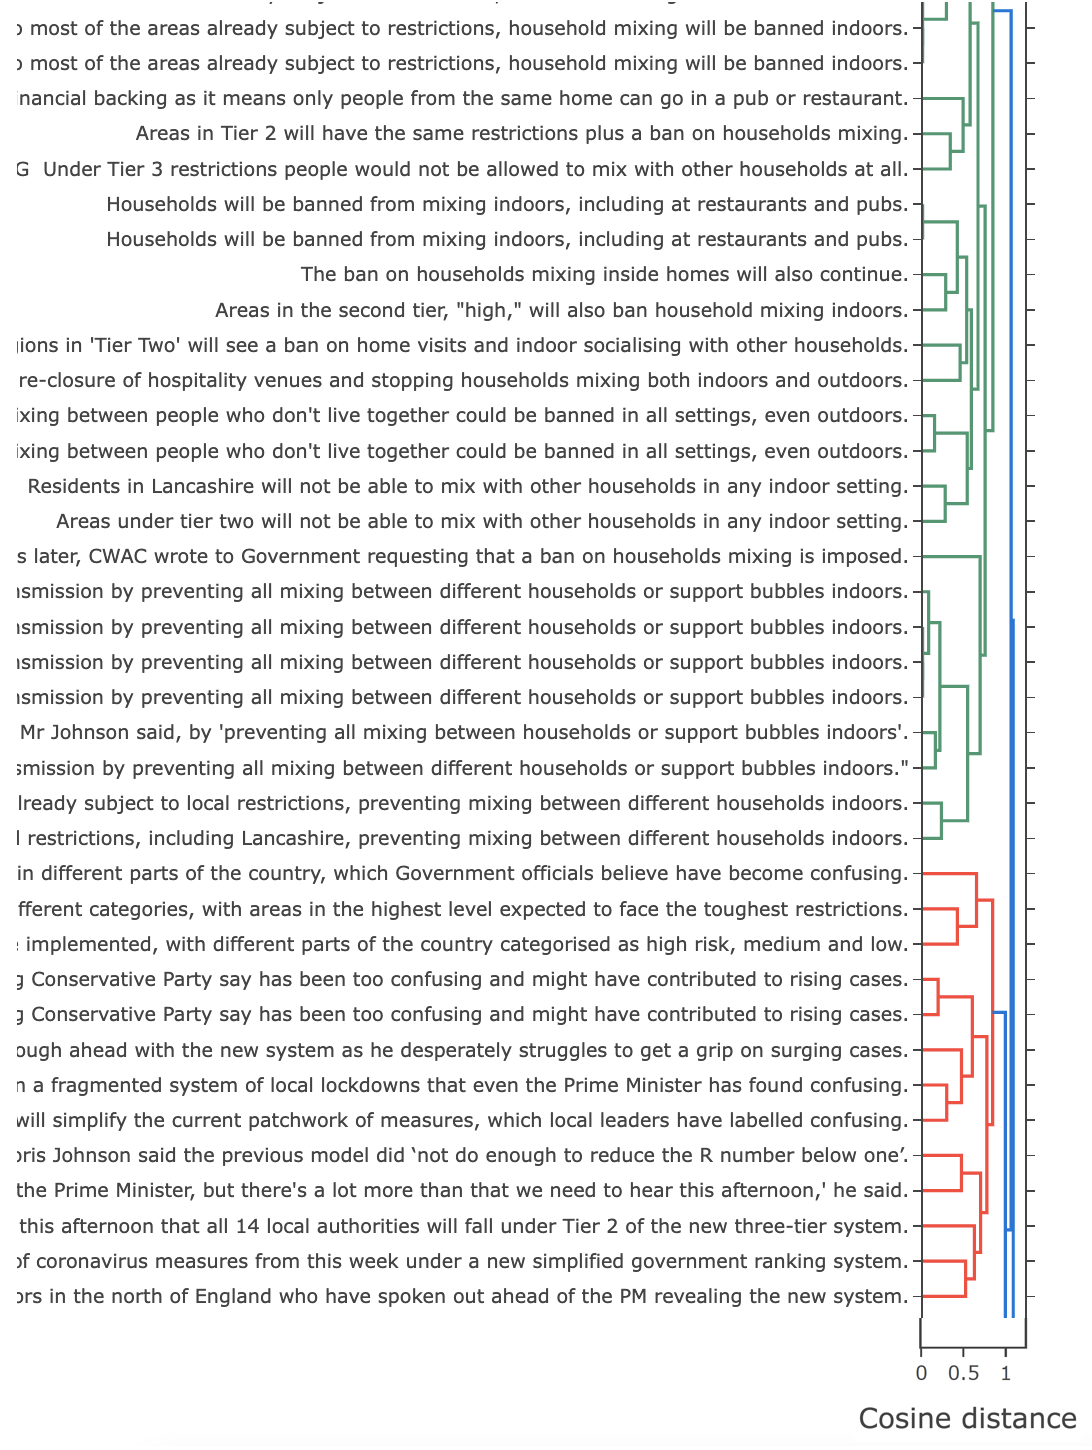
\includegraphics[width=\linewidth]{figures/dendrogram_high_legend.png}
    \caption{Partial dendrogram showing sentences merged by increasing distance.}
    \label{fig:dendrogram}
\end{figure}
% \todoHA{Put in a page by itself}

Using this type of inspection, we can decide specific threshold values that make ``similar enough" sentences go into the same cluster, while keeping other sentences in other clusters.
%we can see what is the required similarity to make two pairs of sentences be in the same cluster.
% \todo{some observations about the distance values and threshold}

% 3. extract degree of uniqueness of words (from pairwise to clusterwise, with bag-of-words or difftool (order matters, duplicates))
% second motivation: highlight the different words and their uniqueness
With this method, we can create sentence clusters that are very similar in their semantic content, but at the same time have linguistic changes. This is a joined effect of having models that deliver a better similarity metric and also of applying a weighted-similarity approach when building the clusters and not just a binary approach (as done instead with a cliquing algorithm instead of clustering ones).

\begin{figure}[!htbp]
    \centering
    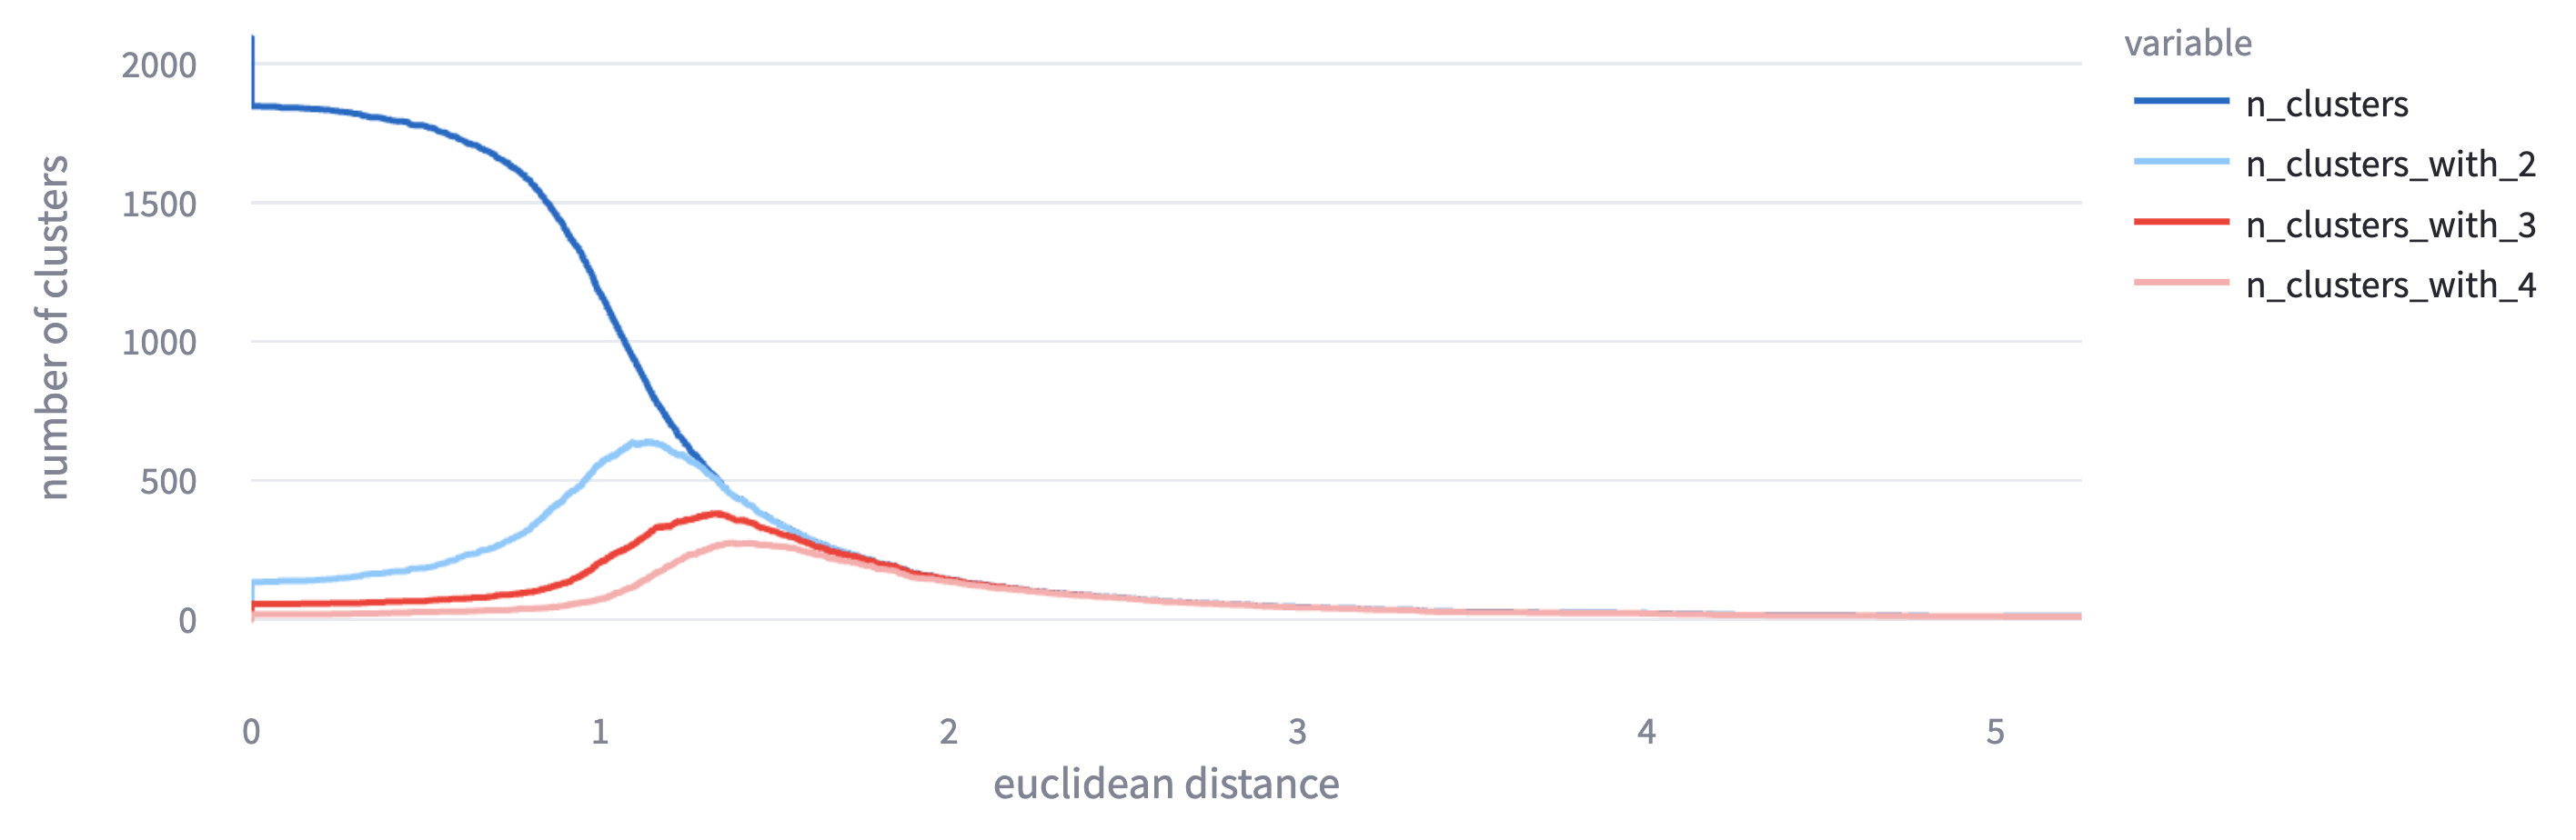
\includegraphics[width=\linewidth]{figures/clusters_count_by_threshold_bigger_2.png}
    \caption{
    Clusters of different minimal sizes with increasing distance thresholds.
    %Number of clusters (with minimal size of 1,2,3,4) plotted when the distance threshold varies. The blue line counts also for sentences that are on their own, while the others lines are more and more stricter with the number of sentences per group to be counted.
    }
    \label{fig:clusers_count_by_threshold}
\end{figure}
% \todo{improve figure: re-export, set limits, scale}
In Figure~\ref{fig:clusers_count_by_threshold} we see how the number of clusters evolves when we increase the similarity threshold. 
The dark blue line indicates all clusters, counting also clusters with just one sentence inside.
On the blue line, we notice a steep drop at distance next to $0$: this denotes that there are lots of sentences that are identical or just differ in punctuation.
A second drop happens around the Euclidean distance of 1.
Then, with the other lines, we represent clusters that have stricter conditions in terms of the minimal number of sentences per cluster. We respectively only count clusters with 2, 3 and 4 sentences minimum.
All these lines have a similar behaviour: with the distance increasing, they increase to reach a maximum (because new clusters are formed satisfying the minimum number of sentences) and then decrease again (because the clusters are merged together, so they are less). 
The peak is reached with Euclidean distance around $1.2$.
Notice that with respect to the previous dendrogram plot, here we are using Euclidean distance to show values less compacted together.
The value of $1.2$ Euclidean is observed across the different headlines to consistently provide clusters with a good variation of terms but still having a strong semantic connection (e.g., same details, same entities mentioned).
Therefore, we use this value in the following Subsection~\ref{sec:cgs_clustering_and_differences_uniqueness}.

% By also inspecting several dendrograms, we consistently notice that around that interval, $0.55-0.65$ Euclidean distance, we are able to capture good variations on the surface form but the meaning of the sentences keeps similar.
% Therefore, we select the value of $0.6$ as our threshold for the next subsection~\ref{sec:cgs_clustering_and_differences_uniqueness} (the example shown in it have this parameter).


% \todo{How do we know this is better than cliques? Ground truth of clusters is not available. A benchmark test would be required to claim superiority. Do we need to repeat the initial experiment with this clustering instead of cliquing?}
% \todoHA{Important question to be discussed. Need to evaluate, if not quantitatively then qualitatively}
% \todoAW{Does such a benchmark test exist anywhere? eg. for other domains?}
From a qualitative analysis of the generated clusters, we find that this methodology produces better sentence clusters with respect to the method described in Section~\ref{sec:cgs_cross_referencing}.
We do not find many examples of sentences belonging to the wrong cluster, and we are able to find word variations that do not cause a major change in meaning.

With the sentence clusters produced, we move to the following Section, where we analyse the variations at the word level.

\subsection{\statusgreen Term Uniqueness}
\label{sec:cgs_clustering_and_differences_uniqueness}

With the outputs of the sentence clustering from the previous section~\ref{sec:cgs_clustering_and_differences_hierarchical}, we want now to take these sentences, which should be similar in the meaning but with some variations on the linguistical form, and analyse how they overlap or not in the terms used.

% What we want to achieve, is to have a good way to analyse the fine-grained differences between the extracted similar sentences.\todoHA{What? What's the final goal?}
Therefore, our final goal for this experiment is to compute the uniqueness of words across multiple variations of describing the same detail.
One news source may be using completely different terms from the others, or share with others the same terminology.
This word-level analysis completes the corroboration and omission analysis, which instead is performed at the sentence level.

To facilitate an analysis of the differences, we experimented with different methods of highlighting the uniqueness of the words in a cluster.
Inspired by software engineering tools, we first tried with algorithms based on \texttt{diff}~\citep{myers1986ano}.
% Diff (also coming in UNIX distributions under the \texttt{diff} tool)
\texttt{Diff} is a great algorithm and UNIX tool for comparing different modified versions of the same document.
This algorithm is also able to detect changes in the position or ordering of elements. This aspect is not very important in our analysis, because natural language is more flexible and reordering phrases and sub-phrases should not be accounted for in our analysis. So with the relaxed constraint on the position of the words, we moved to a measure of term uniqueness based merely on the words appearing or not in the considered sentences. For this reason, we named this comparison \texttt{set-based} instead of \texttt{diff-based} because we treat the words for each sentence as a set (without considering the position and repetitions of words).
Although we do not consider repeated words in a sentence as modifying the uniqueness of terms, we will still take into consideration repetition as a persuasive technique in the next chapter.

We therefore define a scale of uniqueness in the following way:
$$u_w = 1 - \frac{|\set{s_i | s_i \in S \land w \in s_i}|}{|S|}$$
where $S$ is the set of sentences considered, $w$ is the word for which to compute the index. The expression compares the sentences of the current cluster where $w$ appears (numerator) with respect to the cluster size.
A value close to $1$ means that the word is used in just a few sentences in the cluster.

In Figure~\ref{fig:words_uniqueness} we can see an example of this metric applied to a cluster of three sentences.
For each word, the uniqueness score is computed, and then we associate the values to a colour scale.
In this way, we can instantly see the words that are most unique and the ones that instead are repeated across multiple sentences.
In this case, the word ``deceased'', which just appears in one of three sentences, gets assigned a high value of uniqueness ($u = 2/3$). Instead, the word ``surgery'', which appears in all three sentences, has $u = 0$.
% \todoHA{You mean overall or in this example?}

\begin{figure}[!htb]
    \centering
    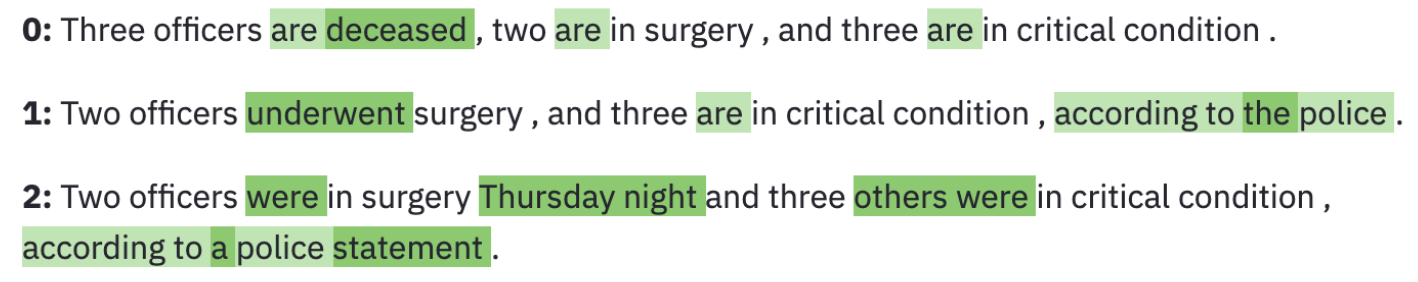
\includegraphics[width=\textwidth]{figures/words_uniqueness.png}
    \caption{A sentence cluster example highlighting the uniqueness of words.}
    \label{fig:words_uniqueness}
\end{figure}


% not only uniqueness, but how it was used to observe variations of terms
This uniqueness was used to inspect around 25 sentence-level clusters that were gathered by using the \acrshort{hac} as described in Section~\ref{sec:cgs_clustering_and_differences_hierarchical}. Helped by the uniqueness degree of the words, we are able to spot the differences between the sentences faster and classify the main types of singular words that change:
\begin{enumerate}
    \item verb tenses: not meaningful in this context
    \item chunks of information at the beginning or end of the sentence. Usually, those pieces are just a matter of segmentation of the sentences (e.g. the reporter actually includes the omitted terms in the next or previous sentence) 
    \item details that are present in some articles and omitted in others (e.g. Figure~\ref{fig:words_uniqueness})
    \item verb choices across synonyms
    \item substantive/adjective choices across synonyms
\end{enumerate}

Across these types of changes, we are particularly interested in the term choices (verbs, substantive, adjectives) as they are the details that may mostly change the message transmitted to the reader.
With this methodology that is only based on similarity and overlap analysis, we are not able to tell more about these term choices. We need external analysis that will be faced in the next Chapter.

\subsection{\statusgreen Meaning of Fine-grained Differences}
% TODO: findings?
The experimentations shown in this section have two directions that seem to be opposing: 
\begin{itemize}
    \item On one side (similarity), create clusters of sentences accordingly to their semantic similarity using a more flexible hierarchical clustering (to capture similar-enough sentences). %(more broad and resistant to changes in the linguistical surface)
    \item On the other side (differences/uniqueness), to be able to extract and see how the word-level details change.
\end{itemize}

It may look like a contradiction, but we need this double analysis to link different sentences that share the same stories and to be able to see the actual differences between them.

With this approach, we are able to see in details which words have changed in sentences coming from different news sources.
With comparison to the approach presented in~\citet{bountouridis2018explaining}, we are now able to see more granularly than just at the document and sentence-level.
There are several ways in which the selection of what to include or to exclude in an article may show facts under a different light. Not only we are able to see which details corroborate or have been omitted (Agenda-setting~\citep{Cohen_1964}), but we identify single terms which can reveal the intention to persuade or to push for a certain interpretation by the writer. Seeing these terms, and the alternative terms used by articles on the same topic, could enable us or the reader to get awareness of the possible influence of the point of view of the writer or news outlet.

However, we see that many variations of terms do not seem to carry any differences in the perspective of the writer. Some others instead, convey a message very differently from a few words. Similarity alone cannot distinguish between them. And in this chapter we do not have the tools to quantify this phenomenon. A we will describe in the last section of this chapter, we need to experiment with the work of persuasion detection (next chapter).



% role of this experiment and outcomes
% This methodology can be used in our framework to help the preparation of the dataset in different steps.
% First of all, during the creation of article couples that have to be compared (using at the article-level the same clustering methodology). In this case, we will need to use a specific threshold that cuts out unrelated articles but at the same time keeps a considerable number of differences on the document level (not too similar because identical articles, that are a lot, are not useful).
% While for the first user study we can exploit hand-curated groups of articles, when doing a larger creation of the dataset we will need to rely on automated techniques.
% This methodology could also be used as support for the annotators, to see both which sentences are most similar, and the words that differ inside. This would make the annotation process faster and easier.

% This experiment needs to be completed, to choose some parameters with better criteria. We want to identify good intervals for the thresholds and parameters (e.g. with euclidean distance around 0.6-1.0 sentences start to have linguistic variations but still very related to the same concepts).

% This experiment evidences the need to explore more on the interpretation of the differences, pushing for the user study of RQ1.1.

% It serves the RQ1.2 as a first implementation of the processing pipeline by making available different articles and their document and sentence-wise relationships. Building on top of these features, we can then develop the methodology for doing the cross-article framing analysis.



\section{\statusgreen Discussion}
\label{sec:cgs_findings}

% From this chapter, we achieved to be able to understand and study when information is unique or shared between different news sources, at different granularities:
% \begin{itemize}
%     \item article-level: finding related articles that cover the same events;\todoHA{Which section shows these results?}
%     \item sentence-level: being able to find the sentences that corroborate, the ones that are unique or omitted;
%     \item word-level: computing the degree of uniqueness of single terms, and observing how single words are changed between multiple sources.
% \end{itemize}

% \todo{I need something to link together this chapter and also need strong findings to conclude it.}

This chapter had several sub-questions, that we discuss separately here, before discussing the overall RQ1:

\begin{enumerate}[label={\textbf{RQ1.\arabic*:}},leftmargin=2cm]
    \item \emph{How are new events reported differently by multiple sources?} News sources present the same event in different ways, including different details that corroborate with other sources, omitting details that other sources instead report, changing the order of presentation of the details. We studied and measured these phenomena in this chapter, but we deem it necessary to study the choice of terms, by investigating what is the reason and what is the effect of deliberate or involuntary choices. We will expand on this in the next Chapter.
    \item \emph{How could we identify what is unique for each report and what is common?} To identify what is unique, common or omitted, it is possible to use the methodology of~\citet{bountouridis2018explaining} to detect omission and corroboration, %(Section~\ref{sec:cgs_cross_referencing})
    which is based on splitting the articles into sentences and comparing them with similarity metrics.
    % We extended the approach to analyse at the word level the variation of terms across multiple related articles, and compute the relative uniqueness of terms 
    We went one step further, by being able to automatically find the specific words that change between multiple news articles, and identify the degree of uniqueness of them (Section~\ref{sec:cgs_clustering_and_differences}). We think that this is potentially beneficial for many downstream tasks, such as showing to the user during annotation tasks or even when consuming news online.
    \item \emph{To what extent can we automatically detect omission and corroboration across multiple articles?} The approach, identified to answer the previous \acrshort{rq}, works better for detecting small differences between articles that have several parts in common. When the articles are too different, for example, if they consider totally different events or if the overlap of terms is too small, it becomes difficult to align the documents with similarity metrics and the results are less meaningful. We also find that our analysis is able to find terms that change but does not give an interpretation of what these changes mean. For example, we cannot currently distinguish between a loaded term versus a more neutral one. For this to be possible, we need the study of persuasion means (as discussed in RQ2).
    \item \emph{Which similarity metrics are best for detecting omission and corroboration?} We underlined in Section~\ref{sec:cgs_similarity} the importance of using semantic similarity metrics that go beyond the binary comparison (equal or different) of terms. In this way, we are more resistant to term changes and can identify better the related sentences across articles.
\end{enumerate}

We can now answer our overall RQ1: \emph{To what extent do news articles about the same events differ?}

After comparing news articles covering the same events, we discovered that they can vary in several ways. Firstly, some articles may omit certain details while others confirm them. Secondly, different terms may be used to express the same detail. While it is relatively straightforward to analyze the first type of difference using similarity metrics, it is not sufficient for understanding the nuances of the second type. We need in this case to analyse the terms involved to go beyond the simple differences.


% The main findings that we have from this chapter are the following:

% \begin{itemize}
%     \item As already denoted by the work of~\citet{bountouridis2018explaining}, we confirm a positive correlation between corroboration and credibility of news outlets and a negative correlation between omission and credibility. We went one step further, by being able to automatically find the specific words that change between multiple news articles, and identify the degree of uniqueness of them. We think that this is beneficial for many downstream tasks, such as showing to the user during annotation tasks or even when consuming news online. %: corroboration correlates positively to credibility of news outlets, omission negatively
%     % \item Extreme left and right corroborate less and omit more? (but needs leaning? No if we just take centrality-extremism)
%     % \item Delta Time of publication: more similar articles are published at similar times, instead the further the time delta the more further they are?
%     % these are more limitations
%     \item Observing similarities between multiple documents is made very difficult by linguistic variations. We experimented with models (e.g. \acrshort{use}) that are more resistant to words that carry similar meanings and are a better fit for doing this type of analysis. %It is not only a matter of what is included and what is excluded. The similarity between sentences is also capturing some linguistic variations more than others (more about the surface and less about the intention).
%     \item We do not have any interpretation of what a change in a document conveys. Something may be written differently just because of random choices, or there can be some hidden reasons and some goals to persuade. The similarity computation, necessary to understand how the documents overlap or not, gives no understanding of the persuasion means and the intention behind specific choices. This will be explored in the next Chapter~\ref{chap:linguistic_persuasion}.
% \end{itemize}



\section{\statusgreen Next}
\label{sec:cgs_next}
% link to next chapter

This chapter gives us some insights into how similar documents are changed and modified across news sources, and how critical corroboration and omission are.

% recap contributions? (done before already)


% open for new chapter
However, what these changes \emph{convey} remains unclear.
It could be that the differences exist for different natures, originating from randomness (each author/source has different jargon, or by casualties).
On the other hand, there could be a purpose that is subtly manifesting through these small choices. This purpose could be to influence the readers, with persuasion or manipulation.

This chapter raised some questions that need to be answered:
What changes between the changed parts? What characterises those differences? How can we characterise the differences quantitatively, describing how they try to persuade the readers? To give an answer to these questions, we need to include in our analysis some concepts of persuasion.

Therefore, in the next chapter we will investigate persuasive language and how it can be computationally quantified. 
